\section{Introduction}
In NASA's Mars 2020 mission, the helicopter \textit{Ingenuity} was deployed to demonstrate the first powered flight on another planet. The helicopter was designed to be a technology demonstrator, and its main goal was to prove that powered flight in the thin Martian atmosphere is possible. By the date of the end of its mission (caused by the rupture of one of the rotor blades), Ingenuity had far exceeded every expectation: originally designed to perform up to five experimental test flights over 30 days, instead it flew for almost three years, performing 72 flights, and traversing more than 14 times the planned distance.

In the upcoming sections of the document we will present a mathematical model of Ingenuity, and we will discuss the control strategies that can be used to stabilize and control it, possibly around a planned trajectory, during flight in the Martian atmosphere. The theoretical results will be validated through simulated experiments.

\subsection{Helicopter structure}
At its core, Ingenuity features a fuselage designed for minimal weight and maximum strength, a sturdy framework for housing critical components such as the avionics, power system, and rotor assembly.

The most prominent feature is its coaxial rotor system, comprising two horizontally-overlapping counter-rotating (to mitigate reaction torque effects) blades, ensuring stability and precise maneuverability during flight. Attached to the rotor system is a central mast, which extends upward from the fuselage.

\begin{figure}[H]
    \centering
    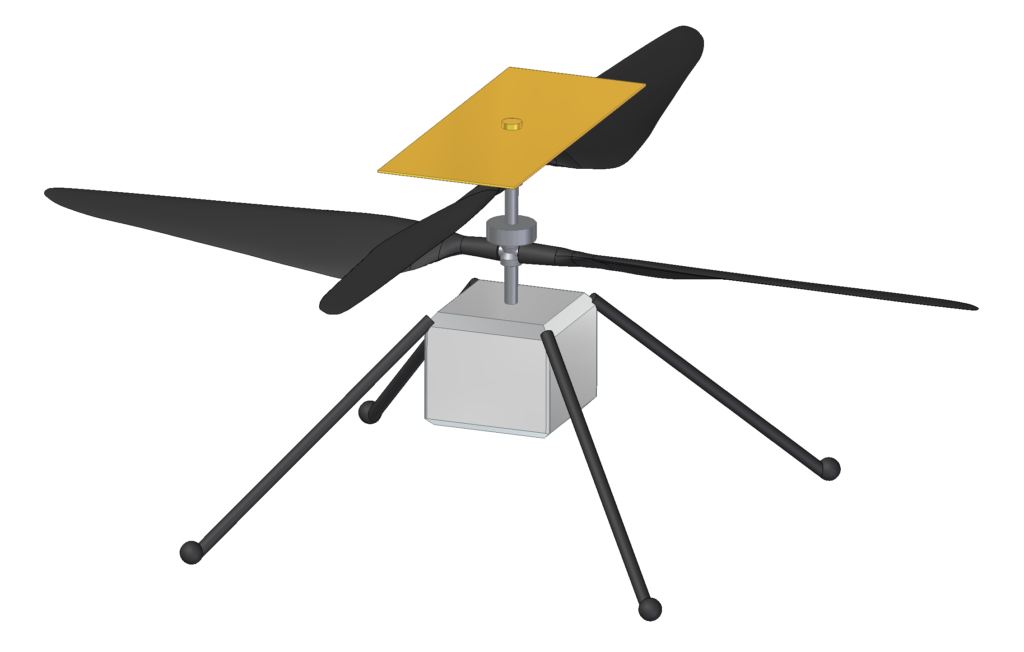
\includegraphics[width=0.7\columnwidth]{figures/ingenuity_render.png}
    \caption{3D render of the Ingenuity Mars Helicopter.}
    \label{fig:ingenuity_render}
\end{figure}

Complementing these is a suite of sensors, cameras, and communication equipment strategically integrated throughout Ingenuity's structure. These instruments enable it to navigate autonomously according to the instructions coming from the base of operation on Earth and capture imagery of the Martian surface.

The main parameters of the helicopter structure model are summarized in Table \ref{tab:ingenuity_parameters}.

\begin{table}[H]
    \centering
    \begin{tabular}{|c|c|c|}
        \hline
        \textbf{Parameter} & \textbf{Symbol} & \textbf{Value} \\
        \hline
        \hline
        Mass & $m$ & \SI{1.8}{\kilogram} \\
        \hline
        Rotor diameter & $2\,r$ & \SI{1.2}{\meter} \\
        \hline
        Blade chord & $c$ & \SI{0.24}{\meter} \\
        \hline
        \begin{tabular}{@{}c@{}}COM - upper\\rotor distance\end{tabular} & $d_{cm, u}$ & \SI{0.10}{\meter} \\
        \hline
        \begin{tabular}{@{}c@{}}COM - lower\\rotor distance\end{tabular} & $d_{cm, l}$ & \SI{0.05}{\meter} \\
        \hline
        Inertia & $I$ & \begin{tabular}{@{}c@{}}$diag(0.210, 0.288, $\\$0.278)$\,\SI{}{\kilogram\square\meter}\end{tabular} \\
        \hline
    \end{tabular}
    \caption{Structural parameters of the Ingenuity model.}
    \label{tab:ingenuity_parameters}
\end{table}

\subsection{Martian environment}
Even though the Martian gravity is only about $38\%$ of the Earth's, its thin atmosphere, composed mainly of carbon dioxide with a ground-level pressure of about $0.6\%$ of the Earth's, makes it difficult for aerial vehicles to fly. The athmospheric model is split in two zones: below and above the altitude of $\SI{7000}{\meter}$. Since Ingenuity only performs low level flights, we are interested in the parameters of the lower layer, whose expressions (with respect to altitude) are summarized in Table \ref{tab:martian_environment}.

\begin{table}[H]
    \centering
    \begin{tabular}{|c|c|c|}
        \hline
        \textbf{Parameter} & \textbf{Sym} & \textbf{Value} \\
        \hline
        \hline
        Gravity & $g$ & \SI{3.71}{\meter\per\square\second} \\
        \hline
        Temperature & $T$ & $-242.1-9.98 \times 10^{-4} \, h$\;\SI{}{\kelvin} \\
        \hline
        Pressure & $p$ & $0.699 \, e^{-0.9 \times 10^{-5} h}$\;\SI{}{\kilo\pascal} \\
        \hline
        Air density & $\rho$ & $p/(0.192\;T)$\;\SI{}{\kilogram\per\cubic\meter} \\
        \hline
    \end{tabular}
    \caption{Martian environment parameters for altitude $h< \SI{7000}{\meter}$.}
    \label{tab:martian_environment}
\end{table}

